\documentclass[conference]{IEEEtran}

\usepackage{cite}
\usepackage{amsmath,amssymb,amsfonts}
\usepackage{graphicx}
\usepackage{booktabs}
\usepackage{multirow}
\usepackage{array}
\usepackage{xcolor}
\usepackage{microtype}
\usepackage{url}
\usepackage[hidelinks]{hyperref}

\graphicspath{{figures/}}
\setlength{\textfloatsep}{8pt plus 1pt minus 2pt}
\setlength{\dbltextfloatsep}{8pt plus 1pt minus 2pt}
\setlength{\intextsep}{8pt plus 1pt minus 2pt}

\begin{document}

\title{Beyond Vanity Metrics: An Empirical Study of Statistical Integrity, Cross-Repository NLP Generalization, and Resolution Predictability in Open-Source Software Ecosystems}

\author{
\IEEEauthorblockN{First Author Name\IEEEauthorrefmark{1}, Second Author Name\IEEEauthorrefmark{1}}
\IEEEauthorblockA{\IEEEauthorrefmark{1}Department of Computer Science and Data Science, Institution Name, City, Country\\
Email: \{first.author, second.author\}@institution.edu}
}

\maketitle

\begin{abstract}
Modern software infrastructure depends heavily on open-source software (OSS) ecosystems hosted on collaborative forges such as GitHub. Yet developers, maintainers, and institutional evaluators still rely overwhelmingly on surface-level popularity counters---stars, forks, and raw open-issue totals---that obscure underlying engineering dynamics, review bottlenecks, and contributor concentration risks. Simultaneously, existing automated repository-intelligence pipelines and machine learning (ML) models frequently suffer from four methodological failures: in-distribution benchmark lock-in that collapses under cross-repository transfer, false precision in creation-time issue resolution forecasting, unguarded statistical telemetry (e.g., null-to-zero coercion, ignored right-censoring, and spurious autocorrelated correlations), and API rate-limit fragility on arbitrary unseen repositories.

This paper presents a comprehensive empirical investigation of OSS telemetry and issue intelligence grounded in a reproducible, rate-budgeted analytical framework (\emph{OpenSourceLens}). Across a curated four-ecosystem benchmark corpus ($N=2{,}328$ issues across \texttt{microsoft/vscode}, \texttt{pytorch/pytorch}, \texttt{kubernetes/kubernetes}, and \texttt{huggingface/transformers}) and three live unseen repositories (\texttt{RocketChat/Rocket.Chat}, \texttt{pallets/click}, and \texttt{git/git}), we evaluate five research questions. First, on 3-class issue triage ($N=385$ holdout), a $0.94$\,MB Platt-calibrated TF-IDF LinearSVC pipeline achieves $81.56\%$ accuracy ($0.8213$ Macro-F1, $1.54$\,ms/sample), outperforming a $66.37$M-parameter fine-tuned DistilBERT encoder ($75.32\%$ accuracy, $0.7586$ Macro-F1, $64.86$\,ms/sample); error diagnostics reveal that $256$-token truncation degrades DistilBERT from $82.65\%$ on short reports to $68.75\%$ on verbose logs, while $96.84\%$ of errors arise from heterogeneous ``other'' spillover. Second, strict Leave-One-Repo-Out (LORO) validation ($N=1{,}922$) exposes severe cross-project domain shift ($29.92\%$ raw mean accuracy), which confidence- and entropy-calibrated abstention elevates to $52.86\%$ mean confident accuracy (up to $69.74\%$ on \texttt{vscode}). Third, compact $384$-dimensional dense embeddings (\texttt{all-MiniLM-L6-v2}) outperform lexical TF-IDF on duplicate and related-issue retrieval ($N=120$ queries; MRR $0.6850$ vs.\ $0.6361$; Hit@1 $64.17\%$ vs.\ $56.67\%$), achieving $100.0\%$ noise rejection and $92.88\%$ label concordance at cosine $\ge 0.70$. Fourth, multivariate econometric analysis proves that repository governance accounts for $71.11\%$ of explainable variance in log-resolution hours, causing within-repository regression $R^2$ to collapse to $[-0.041, +0.181]$ and establishing that non-parametric Kaplan--Meier survival modeling---and at most coarse advisory velocity tiers ($88.11\%$ adjacent $\pm 1$-tier accuracy)---should replace exact-hour forecasts. Finally, live unseen-repository evaluations demonstrate how strict non-zero coercion and explicit confidence penalties transparently capture divergent workflows such as Git's mailing-list governance.
\end{abstract}

\begin{IEEEkeywords}
Open-source software analytics, mining software repositories, cross-repository generalization, calibrated abstention, semantic duplicate retrieval, survival analysis, empirical software engineering.
\end{IEEEkeywords}

% ============================================================================
\section{Introduction}
% ============================================================================

Open-source software (OSS) forms the foundational substrate of contemporary cloud infrastructure, artificial intelligence frameworks, developer tooling, and operating systems. Collaborative coding platforms such as GitHub expose hundreds of millions of public repositories, yet the primary quantitative signals surfaced by forge interfaces remain coarse popularity counters: stargazers, forks, and aggregate open-issue counts. Prior empirical studies demonstrate that GitHub stars primarily reflect social visibility, marketing bursts, and developer bookmarking habits rather than maintenance sustainability, responsiveness, or engineering quality~\cite{borges2018github}. Worse, surface counters routinely distort operational reality---for instance, GitHub's headline ``open issues'' counter conflates pure defect reports with open pull requests, while repositories operating on external patch workflows appear superficially broken when evaluated naively~\cite{kalliamvakou2014promises}.

To bridge this observability gap, the Mining Software Repositories (MSR) and applied machine learning communities have proposed automated health dashboards, issue classifiers~\cite{kallis2019ticket}, duplicate bug detectors~\cite{deshmukh2017duplicate}, and bug fix-time predictors~\cite{giger2010predicting}. However, translating offline research prototypes into trustworthy intelligence across the \emph{entire open-source ecosystem}---where projects vary wildly in language, scale, governance model, and label taxonomy---exposes four persistent methodological failure modes:

\begin{enumerate}
    \item \textbf{In-Distribution Benchmark Lock-In and Taxonomy Shift:} Supervised issue classifiers evaluated via random train/test splits on a fixed set of repositories routinely report high accuracy ($>80\%$) by exploiting repository-specific templates, bot signatures, and label vocabularies. When transferred to unseen repositories with distinct taxonomies, predictive performance degrades precipitously unless guarded by explicit out-of-distribution (OOD) abstention~\cite{geifman2017selective}.
    \item \textbf{False Precision in Resolution-Time Forecasting:} Many analytical studies attempt to predict exact issue-closure duration from creation-time ($t=0$) text and metadata. Such models ignore post-creation maintainer capacity, asynchronous code-review queues, and right-censoring of unresolved issues~\cite{kaplan1958nonparametric}, creating an illusion of precision that erodes practitioner trust when within-project variance remains largely unexplainable.
    \item \textbf{Statistical Malpractice in Repository Telemetry:} Operational OSS metrics frequently coerce missing API fields (such as uncollected commit diffs or disabled issue trackers) into zeros, include incomplete current calendar weeks in velocity trends, conflate automated bots with human maintainers, omit right-censoring from backlog latency estimates, and report cross-domain time-series correlations without guarding against lag-1 serial autocorrelation or multiple hypothesis testing~\cite{benjamini1995controlling}.
    \item \textbf{Opaque Composite Scores and Rate-Limit Fragility:} Arbitrary $0$--$100$ composite ``repository health scores'' hide sample-size limitations behind a single uncalibrated number, while naive full-history crawlers rapidly exhaust public forge API quotas when pointed at arbitrary live repositories.
\end{enumerate}

To systematically investigate these ecosystem-wide phenomena, we formulate five research questions (RQs) and study them through a reproducible statistical and machine learning framework (\emph{OpenSourceLens}) spanning both an offline four-ecosystem benchmark corpus ($N=2{,}328$ issues) and live unseen GitHub repositories:

\begin{itemize}
    \item \textbf{RQ1 (Model Paradigm \& Length Dynamics):} \emph{How do lightweight calibrated lexical models compare against fine-tuned transformer encoders on heterogeneous OSS issue corpora, and what structural document properties drive classification errors?}
    \item \textbf{RQ2 (Cross-Repository Transfer \& Abstention):} \emph{How severely does supervised issue classification degrade under strict Leave-One-Repo-Out (LORO) transfer, and to what extent does calibrated abstention recover actionable precision?}
    \item \textbf{RQ3 (Dense Semantic Retrieval Calibration):} \emph{How effectively do compact dense sentence embeddings outperform lexical retrieval for duplicate and related-issue discovery, and what similarity operating thresholds optimize noise rejection and label concordance?}
    \item \textbf{RQ4 (Determinants \& Feasibility of Resolution Prediction):} \emph{What factor families govern OSS issue resolution latency at creation time ($t=0$), and is exact-hour regression scientifically defensible relative to survival analysis and coarse velocity tiers?}
    \item \textbf{RQ5 (Statistical Integrity on Unseen Live Ecosystems):} \emph{How do rate-budgeted, statistically guarded multi-domain estimators behave across unseen live OSS projects with contrasting governance models?}
\end{itemize}

\textbf{Contributions.} This paper makes four primary contributions to empirical software engineering and applied data science:
\begin{enumerate}
    \item We introduce a mathematically guarded, rate-budgeted multi-domain telemetry methodology (Section~\ref{sec:methodology}) enforcing snapshot isolation, monotonic source revisioning, strict $\texttt{NULL}\neq 0.0$ non-coercion, explicit confidence penalties, and autocorrelation/FDR-guarded cross-domain inference.
    \item We deliver a controlled tri-paradigm NLP evaluation and error audit (Section~\ref{sec:results_cls}) revealing why calibrated full-document TF-IDF outperforms $256$-token DistilBERT on verbose OSS bug reports, and quantify OOD generalization under strict LORO cross-validation with selective abstention (Section~\ref{sec:results_loro}).
    \item We empirically calibrate dense sentence embeddings (\texttt{all-MiniLM-L6-v2}) against lexical retrieval across $120$ benchmark queries and $500$ threshold sweeps (Section~\ref{sec:results_retrieval}), establishing reproducible operating points for per-repository duplicate detection.
    \item We provide an econometric ANOVA and within-repository collapse proof (Section~\ref{sec:results_resolution}) demonstrating why $71.11\%$ of explainable resolution-time variance is repository governance, motivating the quarantine of exact-hour predictions in favor of Kaplan--Meier survival curves, alongside live unseen-repository case studies validating statistical honesty across divergent workflows (Section~\ref{sec:results_live}).
\end{enumerate}

% ============================================================================
\section{Related Work}
% ============================================================================

\subsection{Mining Software Repositories and Ecosystem Health}
Empirical investigations of open-source development trace back to landmark studies of Apache and Mozilla by Mockus et al.~\cite{mockus2002case}, who established quantitative links between core-team concentration, defect density, and release velocity. With GitHub's rise, Gousios et al.~\cite{gousios2014pull} characterized the pull-based development model, showing how review latency, patch size, and contributor track record shape merge outcomes. Simultaneously, Kalliamvakou et al.~\cite{kalliamvakou2014promises} documented critical perils in mining GitHub---including inactive repositories, external merge workflows (e.g., mailing lists), and merged pull requests recorded as closed-unmerged---while Borges and Valente~\cite{borges2018github} demonstrated that star counts measure social popularity rather than engineering rigor. Contributor sustainability has been widely studied through truck/bus factor estimators such as Avelino et al.~\cite{avelino2016truck} and inequality indices (Gini and Lorenz curves). Our work synthesizes these dimensions into a snapshot-isolated, confidence-penalized framework explicitly resistant to the mining perils identified in~\cite{kalliamvakou2014promises}.

\subsection{Automated Issue Classification and Selective Prediction}
Automated issue labeling reduces maintainer triage burden across high-velocity repositories. Kallis et al.~\cite{kallis2019ticket} introduced \emph{Ticket Tagger}, employing fastText over issue titles and bodies to classify GitHub reports into bugs, enhancements, and questions. Subsequent approaches adopted pre-trained transformers such as DistilBERT~\cite{sanh2019distilbert} alongside probability calibration methods such as Platt scaling~\cite{platt1999probabilistic}. However, most benchmarks report pooled in-distribution metrics that mask cross-project domain shift. In machine learning reliability research, Geifman and El-Yaniv~\cite{geifman2017selective} formalized selective classification (prediction with a reject option) to trade coverage for controlled risk. We extend selective abstention to cross-repository OSS issue triage under strict LORO evaluation, quantifying both its gains and its failure boundaries under extreme taxonomy shift.

\subsection{Semantic Duplicate and Related-Issue Retrieval}
Duplicate bug reports fragment maintainer attention and inflate apparent backlogs. Classical lexical models (TF-IDF and BM25) struggle when reporters describe identical defects with distinct phrasing or stack-trace vocabulary. Deep neural retrieval models such as Deshmukh et al.~\cite{deshmukh2017duplicate} leveraged Siamese architectures to capture semantic equivalence. More recently, Sentence-BERT~\cite{reimers2019sentence} and distilled self-attention encoders such as MiniLM~\cite{wang2020minilm} enabled dense $384$-dimensional embeddings with sub-millisecond vector dot-product search on commodity CPUs. We empirically benchmark \texttt{all-MiniLM-L6-v2} against lexical TF-IDF on multi-ecosystem GitHub issues and calibrate explicit cosine operating bands for noise rejection and label concordance.

\subsection{Issue Resolution-Time Analysis and Survival Modeling}
Predicting how long an issue will remain open has attracted extensive attention since Giger et al.~\cite{giger2010predicting}, who showed that early post-creation activity significantly improves fix-time classification over creation-time attributes alone. Crucially, operational repositories contain large fractions of currently open (right-censored) issues; discarding them introduces severe survivorship bias, whereas Kaplan--Meier product-limit estimation~\cite{kaplan1958nonparametric} properly incorporates censored observations. Moreover, testing associations across multiple longitudinal repository series requires rigorous multiple-testing control such as the Benjamini--Hochberg False Discovery Rate (FDR) procedure~\cite{benjamini1995controlling}. Our econometric study rigorously isolates $t=0$ features to test whether exact creation-time resolution prediction is viable across heterogeneous ecosystems.

% ============================================================================
\section{Methodology and Analytical Framework}
\label{sec:methodology}
% ============================================================================

To study OSS ecosystems without falling prey to static-dataset lock-in or statistical distortion, we operationalize our methodology inside a universal analytical engine (\emph{OpenSourceLens}, methodology version \texttt{2026.2}), summarized in Fig.~\ref{fig:framework}. The architecture decouples rate-budgeted data acquisition from snapshot-isolated statistical estimation and generalizable ML/NLP inference.

\begin{figure*}[t]
    \centering
    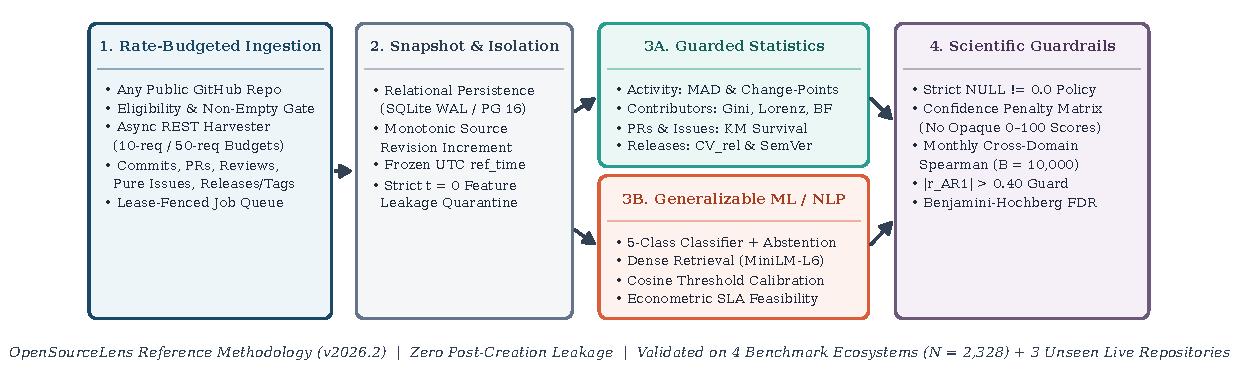
\includegraphics[width=\textwidth]{fig1_framework.pdf}
    \caption{Conceptual and methodological architecture of the guarded OSS analytical framework (\texttt{v2026.2}). Dynamic rate-budgeted acquisition persists normalized entities under monotonic source revisioning and frozen reference time ($\text{ref\_time}$), feeding snapshot-isolated statistical calculators and generalizable ML/NLP models governed by strict non-zero coercion, explicit confidence penalties, and autocorrelation/FDR-protected cross-domain inference.}
    \label{fig:framework}
\end{figure*}

\subsection{Rate-Budgeted Acquisition and Snapshot Isolation}
Analyzing arbitrary public repositories live on GitHub requires respecting strict REST API rate ceilings ($60$\,req/hr unauthenticated; $5{,}000$\,req/hr authenticated). Each repository submission first passes canonical URL validation and public/non-empty eligibility gating (accepting forks and archived repositories with explicit status flags rather than dropping them). An asynchronous harvester enforces a bounded concurrency semaphore ($c_{\max}=2$), inter-request pacing ($100$\,ms), and primary rate-limit halting when remaining quota drops below $10$ requests.

Rather than unbounded crawling, acquisition operates under explicit entity-stream budgets: \emph{Fast Snapshot} ($\le 10$ API requests covering metadata, up to $100$ recent commits, contributors, pull requests, sampled PR reviews, pure issues excluding pull requests, comments, and releases/tags) and \emph{Standard Diagnostic} ($\le 50$ requests extending commit/PR diff lines, inline review comments, and multi-page entity streams). When formal GitHub Releases are absent, the collector automatically falls back to repository git tags.

To guarantee analytical consistency under concurrent updates, ingestion and analytics run via durable, lease-fenced job queues ($\text{lease}=600$\,s, monotonic \texttt{lease\_version} fencing preventing split-brain commits). Every material mutation atomically increments \texttt{analytics\_source\_revision}. Each analytical run opens a pinned read snapshot bound to that revision and freezes a UTC reference timestamp $t_{\text{ref}}$; rows timestamped after $t_{\text{ref}}$ are strictly excluded, ensuring deterministic reproducibility.

\subsection{Core Multi-Domain Statistical Estimators}
All objective measurements are separated from ML/NLP inference across five foundational engineering domains:

\subsubsection{Development Activity}
Trailing commit velocities are computed over rolling day windows ($4$\,w, $12$\,w, $52$\,w) anchored at $t_{\text{ref}}$. To eliminate partial-week distortion, weekly consistency metrics (mean, median, IQR, MAD, and coefficient of variation $\text{CV} = s / \bar{x}$) strictly exclude the ongoing partial UTC week. Rolling anomalous surges and drops are detected via a robust modified $Z$-score over a trailing $6$--$8$ completed-week baseline:
\begin{equation}
    Z_t = \frac{x_t - \operatorname{median}(x_{t-w:t-1})}{\max\!\bigl(1.4826 \cdot \operatorname{MAD}(x_{t-w:t-1}),\, 1.0\bigr)},
\end{equation}
with Poisson floor guardrails, flagging surges at $Z_t \ge 3.0$ and drops at $Z_t \le -2.5$. Structural regime shifts are detected via a single-split maximum between-segment sum-of-squares (\texttt{max\_ssb}) deterministic permutation test ($B=999$, minimum segment length $5$, $p_{\text{perm}} \le 0.01$, $|\Delta\mu| \ge 3.0$). Code churn ($\text{additions}+\text{deletions}$) explicitly reports its non-null \texttt{diff\_coverage\_ratio}.

\subsubsection{Contributor Ecosystem}
Actor identity resolution anchors on immutable \texttt{github\_id} (confidence $1.0$), falling back to unlinked \texttt{git\_email} ($0.7$) without speculative cross-merging, while isolating bot accounts (\texttt{is\_bot} or \texttt{[bot]} suffix) from human concentration metrics. For sorted non-negative human commit counts $x_{(1)} \le \dots \le x_{(n)}$ across $n$ active authors, contribution inequality is quantified by the Gini coefficient:
\begin{equation}
    G = \operatorname{clip}_{[0,1]}\!\left(\frac{2 \sum_{i=1}^{n} i \cdot x_{(i)}}{n \sum_{i=1}^{n} x_i} - \frac{n+1}{n}\right),
\end{equation}
complemented by an $11$-point standardized Lorenz curve, normalized Shannon entropy $H / \log_2 n$, and bus factors $\text{BF}_{50}$ and $\text{BF}_{80}$ (minimum authors accounting for $\ge 50\%$ and $\ge 80\%$ of commits). Retention cohorts are explicitly gated behind verified full-history ingestion to prevent bounded-window selection bias.

\subsubsection{Pull Request and Code-Review Lifecycle}
Human responsiveness is decomposed into three distinct channels excluding self-actions and bots: overall time-to-first-response ($\text{TTFResp}$, minimum elapsed hours across formal reviews, inline diff comments, and conversation comments), formal review latency ($\text{TTFR}_{\text{formal}}$), and inline code-comment latency ($\text{TTFR}_{\text{inline}}$). Merge and abandonment rates, merge latency quantiles ($p_{25}, p_{50}, p_{75}, p_{90}$), diff-size turnaround bins (\emph{small} $0$--$50$, \emph{medium} $51$--$250$, \emph{large} $251$--$1000$, \emph{xl} $>1000$ lines), and reviewer load concentration expose structural review bottlenecks.

\subsubsection{Issue and Backlog Intelligence}
Pure issues are strictly separated from pull requests. Open backlogs are stratified into five aging cohorts ($<7$\,d, $7$--$30$\,d, $31$--$90$\,d, $91$--$365$\,d, $>365$\,d). To avoid survivorship bias from unresolved tickets, both PR and issue lifecycles employ the right-censored Kaplan--Meier product-limit survival estimator~\cite{kaplan1958nonparametric}:
\begin{equation}
    \hat{S}(t) = \prod_{t_i \le t} \left(1 - \frac{d_i}{n_i}\right),
\end{equation}
where $d_i$ denotes resolved items at duration $t_i$, $n_i$ denotes items at risk just prior to $t_i$, and open items are right-censored at $t_{\text{ref}} - t_{\text{created}}$.

\subsubsection{Release Evolution}
Inter-release regularity is measured via $\text{CV}_{\text{release}} = s_{\Delta t} / \bar{\Delta t}$, categorizing repositories as \emph{highly scheduled} ($\le 0.35$), \emph{moderately predictable} ($0.35$--$0.75$), or \emph{event-driven/sporadic} ($>0.75$), alongside Semantic Versioning (SemVer 2.0.0) adoption rates and $14$-day pre-release commit surges relative to prior $60$-day baselines.

\subsection{Cross-Domain Guardrails and Honest Confidence Accounting}
Cross-domain longitudinal relationships are evaluated across three calendar-month aligned pairs: (\texttt{PAIR-01}) monthly code churn vs.\ issue creations, (\texttt{PAIR-02}) monthly median $\text{TTFResp}$ vs.\ PR abandonment rate, and (\texttt{PAIR-03}) monthly commit velocity vs.\ PR merge volume. To prevent spurious macro-correlations, every pair must pass three sequential statistical gates: (i) minimum sample overlap $K \ge 12$ non-null months; (ii) lag-1 serial autocorrelation screening rejecting permutation testing whenever $|r_{\text{AR1}}| > 0.40$ on either series; and (iii) exact two-tailed Monte Carlo rank permutation ($B=10{,}000$) followed by Benjamini--Hochberg FDR correction~\cite{benjamini1995controlling} at $q \le 0.05$.

Finally, the engine enforces a strict \emph{no fabricated zeros} invariant: uncollected streams or disabled GitHub features remain \texttt{NULL} with explicit status codes (\texttt{empty}, \texttt{insufficient}, \texttt{degraded}). Rather than emitting opaque $0$--$100$ health scores, each domain $d$ begins at $1.0$ and incurs transparent additive penalties $P_d \in [0, 1]$ for bounded samples or empty coverage, yielding an overall telemetry confidence score $\bar{C} = \frac{1}{D}\sum_{d=1}^{D}\max(0, 1 - P_d)$ banded into \emph{high} ($\ge 0.80$), \emph{medium} ($0.60$--$0.79$), \emph{low} ($0.40$--$0.59$), and \emph{unreliable} ($<0.40$).

\subsection{Generalizable ML/NLP Pipelines and Selective Abstention}
Machine learning is reserved exclusively for unstructured text and empirical feasibility assessment:
\begin{enumerate}
    \item \textbf{Calibrated Issue Classification with Abstention:} Text undergoes domain-aware normalization replacing code fences, inline code, URLs, mentions, and issue references with structural placeholders, followed by $3\times$ title weighting relative to body text. For generalizable 5-class triage (\texttt{bug}, \texttt{feature}, \texttt{documentation}, \texttt{question}, \texttt{other}), we train a balanced sublinear TF-IDF ($1$--$2$-gram, up to $10{,}000$ features) multinomial logistic model equipped with a dual abstention rule. Given posterior distribution $\mathbf{p} = (p_1, \dots, p_K)$ and normalized Shannon entropy
    \begin{equation}
        \tilde{H}(\mathbf{p}) = -\frac{1}{\ln K}\sum_{c=1}^{K} p_c \ln p_c,
    \end{equation}
    the classifier abstains (\texttt{uncertain}) whenever $\max_c p_c < \tau_{\text{conf}}$ ($\tau_{\text{conf}}=0.40$) or entropy exceeds $\tau_H$, trading coverage for OOD precision~\cite{geifman2017selective}.
    \item \textbf{Per-Repository Dense Semantic Retrieval:} Issues are encoded into $384$-dimensional $L_2$-normalized vectors via \texttt{sentence-transformers/all-MiniLM-L6-v2}~\cite{reimers2019sentence,wang2020minilm} and persisted per repository as compact $1{,}536$-byte IEEE-754 \texttt{float32} binary blobs. Cosine similarity reduces to a vectorized dot product $\mathbf{q}^\top \mathbf{E}^\top$, eliminating external vector-database dependencies while scoping duplicate discovery strictly to each target repository.
    \item \textbf{Leakage-Free Resolution Econometrics:} All $28$ predictors for resolution-time modeling are strictly quarantined to creation time ($t=0$), excluding comment counts, post-creation reactions, and state-change events.
\end{enumerate}

% ============================================================================
\section{Benchmark Corpus and Experimental Protocol}
\label{sec:setup}
% ============================================================================

\subsection{Multi-Ecosystem Benchmark Dataset}
To ensure cross-domain representativeness across programming languages, architectures, and governance styles, we constructed a standardized benchmark corpus of $N = 2{,}328$ GitHub issues spanning four major ecosystems:
\begin{itemize}
    \item \texttt{kubernetes/kubernetes} (Go, cloud orchestration): $599$ issues ($299$ closed, $300$ open; median resolution $141.22$\,h).
    \item \texttt{pytorch/pytorch} (Python/C++, deep learning): $598$ issues ($298$ closed, $300$ open; median resolution $62.37$\,h).
    \item \texttt{huggingface/transformers} (Python, NLP/AI): $595$ issues ($296$ closed, $299$ open; median resolution $38.75$\,h).
    \item \texttt{microsoft/vscode} (TypeScript, IDE/developer tools): $536$ issues ($242$ closed, $294$ open; median resolution $7.71$\,h).
\end{itemize}
Across the corpus, $1{,}135$ issues ($48.8\%$) are closed and $1{,}193$ ($51.2\%$) remain right-censored open. Repository-specific labels ($6{,}361$ raw label assignments) were harmonized into five canonical categories plus unlabeled: \texttt{bug} ($800$), \texttt{other} ($761$), \texttt{feature} ($340$), \texttt{documentation} ($17$), \texttt{question} ($4$), and \texttt{unlabeled} ($406$). The extreme scarcity of explicit \texttt{documentation} and \texttt{question} labels reflects real-world GitHub labeling practice, where repositories frequently route usage questions outside issue trackers or fold documentation defects under general categories.

\subsection{Evaluation Protocols}
\begin{enumerate}
    \item \textbf{In-Distribution Tri-Paradigm Classification (RQ1):} Evaluated on the $3$-class core subset (\texttt{bug}, \texttt{feature}, \texttt{other}) using a stratified $70/15/15$ split yielding $N=385$ held-out test issues ($160$ bug, $68$ feature, $157$ other). We compare TF-IDF + Logistic Regression, TF-IDF + LinearSVC, an enhanced Classical NLP Pipeline ($3\times$ title weighting + domain preprocessing + Platt-calibrated LinearSVC~\cite{platt1999probabilistic}), and fine-tuned \texttt{distilbert-base-uncased} ($66{,}365{,}187$ parameters, $3$ epochs, max $256$ WordPiece tokens). All latency benchmarks are measured on CPU.
    \item \textbf{Strict Leave-One-Repo-Out Generalization (RQ2):} Evaluated across all $N=1{,}922$ canonically labeled issues in $4$ folds where three repositories form the training set and the fourth unseen repository serves exclusively as the test set, reporting raw accuracy, Macro-F1, abstention rate, confident coverage, and confident accuracy at $\tau_{\text{conf}}=0.40$.
    \item \textbf{Semantic Retrieval and Threshold Calibration (RQ3):} Evaluated over $N=120$ queries ($60$ explicit cross-reference pairs and $60$ textual perturbations) comparing \texttt{all-MiniLM-L6-v2} against a lexical TF-IDF baseline using MRR, Hit@$k$, and NDCG@$k$. Operating thresholds ($\tau \in \{0.45, 0.55, 0.70\}$) are calibrated across a $500$-sample similarity sweep measuring cross-repository noise rejection and canonical label concordance.
    \item \textbf{Resolution Econometrics and Modeling (RQ4):} Non-parametric distributional tests (Kruskal--Wallis $H$, Mann--Whitney $U$) and multivariate OLS with Type-III ANOVA variance decomposition are computed over all $N=1{,}135$ closed issues using $\ln(\text{hours}+1)$ and $28$ strictly $t=0$ predictors spanning five factor families (Repository Governance, Structural Complexity, Technical Evidence, Issue Typology, Temporal \& Author Context). Predictive regressors (Dummy, Ridge, Random Forest, Gradient Boosting) and $4$-tier velocity classifiers ($<1$\,d, $1$--$7$\,d, $7$--$30$\,d, $30+$\,d) are evaluated on an $80/20$ holdout split ($908$ train / $227$ test), audited both pooled and per-repository.
    \item \textbf{Live Unseen-Repository Validation (RQ5):} End-to-end dynamic ingestion and snapshot-isolated analytics are executed against three diverse unseen repositories outside the training benchmark: \texttt{RocketChat/Rocket.Chat}, \texttt{pallets/click}, and \texttt{git/git}.
\end{enumerate}

% ============================================================================
\section{Empirical Results and Analysis}
\label{sec:results}
% ============================================================================

\subsection{RQ1: Tri-Paradigm Issue Classification and Truncation Diagnostics}
\label{sec:results_cls}

Table~\ref{tab:classification} summarizes the head-to-head comparison across classical linear baselines, the enhanced calibrated classical pipeline, and fine-tuned DistilBERT on the $N=385$ held-out test set. Contrary to the common assumption that fine-tuned transformers automatically dominate text classification on technical corpora, the lightweight Platt-calibrated TF-IDF LinearSVC pipeline achieves the highest performance across every quality and efficiency metric: \textbf{$81.56\%$ accuracy}, \textbf{$0.8213$ Macro-F1}, \textbf{$0.9120$ Macro ROC-AUC}, and \textbf{$0.0893$ Brier score} at \textbf{$1.54$\,ms/sample} ($0.94$\,MB artifact). Fine-tuned DistilBERT trails by $-6.24$ percentage points in accuracy ($75.32\%$) and $-0.0627$ in Macro-F1 ($0.7586$), while requiring $42.1\times$ higher CPU inference latency ($64.86$\,ms/sample) and $285\times$ larger model storage ($267.8$\,MB).

\begin{table}[t]
\centering
\caption{In-Distribution Tri-Paradigm Issue Classification Benchmark ($N=385$ Holdout, 3 Canonical Classes, CPU Inference)}
\label{tab:classification}
\setlength{\tabcolsep}{3.2pt}
\resizebox{\columnwidth}{!}{%
\begin{tabular}{@{}lcccccc@{}}
\toprule
\textbf{Model Paradigm} & \textbf{Acc.} & \textbf{Mac.} & \textbf{ROC-} & \textbf{Brier} & \textbf{Lat.} & \textbf{Size} \\
 & \textbf{(\%)} & \textbf{F1} & \textbf{AUC} & \textbf{Score} & \textbf{(ms)} & \textbf{(MB)} \\
\midrule
TF-IDF + LogReg & 81.04 & 0.8109 & --- & 0.2699 & --- & 0.48 \\
TF-IDF + LinearSVC & 81.30 & 0.8114 & --- & 0.2721 & 1.20 & 0.48 \\
\textbf{Calib.\ Classical NLP}$^\dagger$ & \textbf{81.56} & \textbf{0.8213} & \textbf{0.9120} & \textbf{0.0893} & \textbf{1.54} & \textbf{0.94} \\
Fine-Tuned DistilBERT & 75.32 & 0.7586 & 0.9005 & 0.3413 & 64.86 & 267.8 \\
\bottomrule
\multicolumn{7}{@{}l@{}}{\footnotesize $^\dagger$Title $3\times$ weighting + domain preprocessing + Platt-scaled LinearSVC.}
\end{tabular}%
}
\end{table}

\begin{figure*}[t]
    \centering
    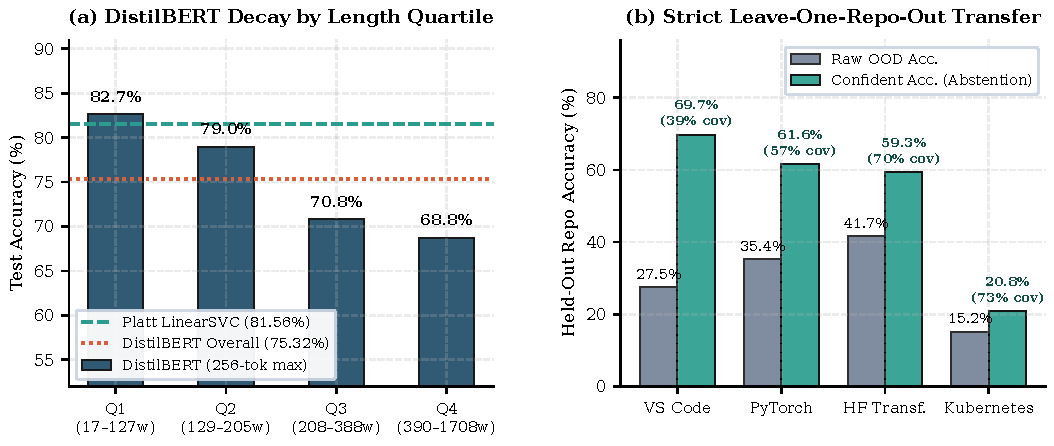
\includegraphics[width=0.92\textwidth]{fig2_classification_loro.pdf}
    \caption{Empirical dynamics of OSS issue classification. (a) Fine-tuned DistilBERT outperforms classical NLP on short issues (Q1: $82.65\%$) but suffers steep accuracy decay as verbose technical logs exceed the $256$-token window (Q4: $68.75\%$). (b) Under strict Leave-One-Repo-Out (LORO) evaluation across $N=1{,}922$ issues, calibrated abstention ($\tau_{\text{conf}}=0.40$) substantially lifts confident accuracy on unseen repositories while exposing severe taxonomy divergence on \texttt{kubernetes/kubernetes}.}
    \label{fig:classification}
\end{figure*}

A rigorous error audit of all $95$ DistilBERT misclassifications ($24.68\%$ error rate) uncovers two structural causes specific to open-source bug trackers:
\begin{enumerate}
    \item \textbf{Token-Window Truncation of Verbose Logs:} As illustrated in Fig.~\ref{fig:classification}(a), DistilBERT achieves \textbf{$82.65\%$ accuracy} on short issues (Q1: $17$--$127$ words, $n=98$)---actually \emph{surpassing} the classical pipeline---but degrades monotonically across length quartiles: $78.95\%$ in Q2 ($129$--$205$w), $70.83\%$ in Q3 ($208$--$388$w), and \textbf{$68.75\%$} in Q4 ($390$--$1{,}708$w). Across the $150$-word truncation boundary ($\approx 256$ subword tokens), error rate jumps from $19.33\%$ ($23/119$) on non-truncated issues to $27.07\%$ ($72/266$) on truncated issues ($53$ of $95$ errors attributed to verbose log truncation). Conversely, sublinear TF-IDF ingests the entire document without truncation, preserving lexical markers buried beneath issue templates and stack traces.
    \item \textbf{Heterogeneous ``Other'' Spillover and Intrinsic Label Noise:} Remarkably, \textbf{$96.84\%$ ($92/95$)} of DistilBERT's errors involve the catch-all \texttt{other} class ($34$ \texttt{other}$\to$\texttt{bug}, $31$ \texttt{bug}$\to$\texttt{other}, $15$ \texttt{other}$\to$\texttt{feature}, $12$ \texttt{feature}$\to$\texttt{other}), whereas direct \texttt{bug}$\leftrightarrow$\texttt{feature} confusion accounts for only \textbf{$3.16\%$ ($3/95$)}. Cross-model agreement between the classical champion and DistilBERT is $84.42\%$ (Cohen's $\kappa = 0.752$): both models succeed on $71.17\%$ ($274$), both fail on $14.29\%$ ($55$ intrinsically ambiguous or noisily labeled tickets), classical-only succeeds on $10.39\%$ ($40$), and DistilBERT-only succeeds on $4.16\%$ ($16$), placing the oracle ensemble ceiling at $85.71\%$.
\end{enumerate}

\textbf{Finding 1:} \emph{On real-world GitHub issues dominated by templates and verbose stack traces, full-document calibrated lexical models outperform $256$-token transformers at $42\times$ lower CPU latency; transformer advantage holds only on concise issues ($<128$ words).}

\subsection{RQ2: Out-of-Distribution Generalization via LORO and Abstention}
\label{sec:results_loro}

In-distribution benchmarks systematically overstate real-world transferability because training and test sets share repository-specific jargon and template structures. Table~\ref{tab:loro} and Fig.~\ref{fig:classification}(b) present strict 5-class Leave-One-Repo-Out (LORO) evaluation across all $N=1{,}922$ labeled issues using our generalizable classifier with calibrated abstention ($\tau_{\text{conf}} = 0.40$).

\begin{table}[t]
\centering
\caption{Strict 5-Class Leave-One-Repo-Out (LORO) Evaluation with Calibrated Abstention ($N=1{,}922$, $\tau_{\text{conf}}=0.40$)}
\label{tab:loro}
\setlength{\tabcolsep}{3.6pt}
\begin{tabular}{@{}lcccccc@{}}
\toprule
\textbf{Held-Out Repo} & \textbf{$N$} & \textbf{Raw} & \textbf{Raw} & \textbf{Abst.} & \textbf{Cov.} & \textbf{Conf.} \\
 & & \textbf{Acc.} & \textbf{M-F1} & \textbf{Rate} & \textbf{(\%)} & \textbf{Acc.} \\
\midrule
\texttt{microsoft/vscode} & 386 & 27.46 & 0.2221 & 60.62 & 39.38 & \textbf{69.74} \\
\texttt{pytorch/pytorch} & 594 & 35.35 & 0.2511 & 42.59 & 57.41 & \textbf{61.58} \\
\texttt{hf/transformers} & 343 & 41.69 & 0.1825 & 29.74 & 70.26 & \textbf{59.34} \\
\texttt{k8s/kubernetes} & 599 & 15.19 & 0.1291 & 26.88 & 73.12 & 20.78 \\
\midrule
\textbf{Macro Mean} & \textbf{1,922} & \textbf{29.92} & \textbf{0.1962} & \textbf{39.96} & \textbf{60.04} & \textbf{52.86} \\
\bottomrule
\end{tabular}
\end{table}

Without abstention, zero-shot OOD accuracy collapses from $\approx 81\%$ in-distribution to a mean of \textbf{$29.92\%$} ($0.1962$ Macro-F1), exposing how heavily standard classifiers overfit to project-specific labeling dialects. Activating calibrated abstention lifts mean confident accuracy by $+22.94$ percentage points to \textbf{$52.86\%$} at $60.04\%$ mean coverage: on \texttt{microsoft/vscode}, abstaining on $60.62\%$ of uncertain tickets raises accuracy from $27.46\%$ to \textbf{$69.74\%$}; on \texttt{pytorch/pytorch} from $35.35\%$ to \textbf{$61.58\%$}; and on \texttt{huggingface/transformers} from $41.69\%$ to \textbf{$59.34\%$} at $70.26\%$ coverage.

Crucially, \texttt{kubernetes/kubernetes} reveals an instructive failure mode: confident accuracy reaches only $20.78\%$ ($73.12\%$ coverage). Inspection shows that Kubernetes employs highly formalized Special Interest Group (\texttt{sig/*}) and \texttt{kind/*} bot-triaged templates whose lexical signatures diverge sharply from IDE and ML repositories, causing miscalibrated overconfidence on unseen \texttt{other}-class administrative tickets.

\textbf{Finding 2:} \emph{Cross-repository transfer exposes severe taxonomy shift invisible in pooled splits. Selective abstention recovers $+18$ to $+42$ percentage points of accuracy on unseen ecosystems, yet extreme governance dialects (e.g., Kubernetes) require broader multi-repo pretraining or unsupervised domain adaptation.}

\subsection{RQ3: Dense Semantic Retrieval and Threshold Calibration}
\label{sec:results_retrieval}

Table~\ref{tab:retrieval} and Fig.~\ref{fig:retrieval}(a) compare dense $384$-dimensional \texttt{all-MiniLM-L6-v2} embeddings against a classical lexical TF-IDF baseline across $N=120$ benchmark queries ($60$ cross-referenced issues and $60$ textual perturbations). Dense semantic retrieval consistently improves top-rank precision: \textbf{MRR rises from $0.6361$ to $0.6850$ ($+4.89$ pp)}, \textbf{Hit@1 jumps from $56.67\%$ to $64.17\%$ ($+7.50$ pp)}, \textbf{NDCG@5 improves from $0.6572$ to $0.6890$ ($+3.18$ pp)}, and \textbf{Hit@10 reaches $80.83\%$} ($97/120$ queries retrieved).

\begin{table}[t]
\centering
\caption{Dense Semantic vs.\ Lexical Retrieval ($N=120$ Queries) and Calibrated Cosine Operating Points ($N=500$ Sweep)}
\label{tab:retrieval}
\setlength{\tabcolsep}{3.2pt}
\resizebox{\columnwidth}{!}{%
\begin{tabular}{@{}lcccccc@{}}
\toprule
\multicolumn{7}{c}{\textbf{Panel A: Retrieval Quality Benchmark ($N=120$ Queries)}} \\
\midrule
\textbf{Method} & \textbf{MRR} & \textbf{Hit@1} & \textbf{Hit@3} & \textbf{Hit@5} & \textbf{Hit@10} & \textbf{NDCG@5} \\
\midrule
Lexical TF-IDF & 0.6361 & 56.67\% & 69.17\% & \textbf{74.17\%} & 79.17\% & 0.6572 \\
\textbf{all-MiniLM-L6-v2} & \textbf{0.6850} & \textbf{64.17\%} & \textbf{69.17\%} & 73.33\% & \textbf{80.83\%} & \textbf{0.6890} \\
\midrule
\multicolumn{7}{c}{\textbf{Panel B: Calibrated Operating Thresholds (\texttt{all-MiniLM-L6-v2})}} \\
\midrule
\textbf{Operating Tier} & \textbf{$\tau_{\cos}$} & \multicolumn{2}{c}{\textbf{Noise Rej.}} & \multicolumn{2}{c}{\textbf{Label Conc.}} & \textbf{Top-1 Dist.} \\
\midrule
Low / Weak & $\ge 0.45$ & \multicolumn{2}{c}{98.67\%} & \multicolumn{2}{c}{56.83\%} & 10.0\% \\
Medium Related & $\ge 0.55$ & \multicolumn{2}{c}{99.93\%} & \multicolumn{2}{c}{70.21\%} & 50.0\% \\
\textbf{High Duplicate} & $\mathbf{\ge 0.70}$ & \multicolumn{2}{c}{\textbf{100.00\%}} & \multicolumn{2}{c}{\textbf{92.88\%}} & \textbf{39.0\%} \\
\bottomrule
\end{tabular}%
}
\end{table}

\begin{figure*}[t]
    \centering
    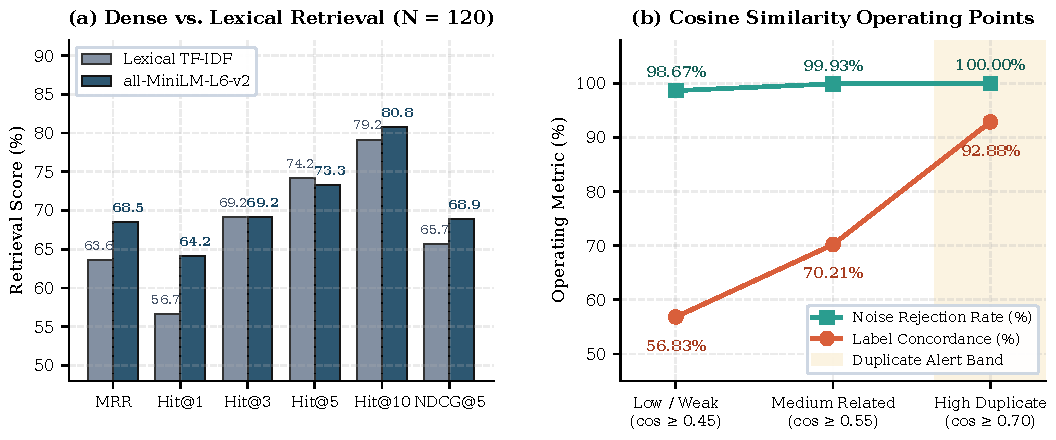
\includegraphics[width=0.92\textwidth]{fig3_retrieval_calibration.pdf}
    \caption{Semantic duplicate retrieval evaluation. (a) Compact $384$-d \texttt{all-MiniLM-L6-v2} embeddings outperform lexical TF-IDF on top-rank precision (Hit@1 $+7.5$ pp, MRR $+4.9$ pp). (b) Calibrated cosine thresholds across $500$ sweep samples establish $\cos \ge 0.70$ as a high-precision duplicate band ($100.0\%$ cross-repo noise rejection and $92.88\%$ canonical label concordance).}
    \label{fig:retrieval}
\end{figure*}

Operationally, encoding all $2{,}328$ benchmark issues on CPU completes in $30.56$--$39.77$\,s ($58.5$--$76.2$\,samples/s) with a total memory footprint of just \textbf{$3.41$\,MB} ($1{,}536$ bytes/issue). Pre-indexed top-$5$ vector dot-product search executes in \textbf{$0.78$\,ms} ($1{,}283.7$\,QPS), while live text-to-vector queries complete in \textbf{$18.98$\,ms} ($52.7$\,QPS). Panel B of Table~\ref{tab:retrieval} and Fig.~\ref{fig:retrieval}(b) establish calibrated cosine operating points: at $\cos \ge 0.70$, cross-repository false-positive noise rejection reaches \textbf{$100.0\%$} with \textbf{$92.88\%$} canonical label concordance, whereas $\cos \in [0.55, 0.70)$ serves as a clean ``related context'' band ($99.93\%$ noise rejection, $70.21\%$ concordance).

\textbf{Finding 3:} \emph{Compact $384$-d dense embeddings stored as native relational BLOBs deliver superior top-rank duplicate discovery at sub-millisecond vector query latency, with $\cos \ge 0.70$ providing a zero-noise duplicate alert band.}

\subsection{RQ4: Resolution-Time Econometrics and Predictability Limits}
\label{sec:results_resolution}

Raw issue resolution durations across the $N=1{,}135$ closed benchmark issues exhibit severe heavy-tailed skewness: mean $200.47$\,h vs.\ median $42.08$\,h ($\text{SD}=349.66$\,h, $\text{IQR}=195.47$\,h, skewness $S=2.616$, excess kurtosis $7.246$, $p_{90}=644.73$\,h). Applying a $\ln(\text{hours}+1)$ transformation stabilizes skewness to $-0.158$. Non-parametric hypothesis tests reveal stark structural stratification:
\begin{itemize}
    \item \textbf{By Repository:} Kruskal--Wallis $H = 224.95$, $p = 1.71 \times 10^{-48}$ (medians span $18.3\times$: \texttt{vscode} $7.71$\,h, \texttt{transformers} $38.75$\,h, \texttt{pytorch} $62.37$\,h, \texttt{kubernetes} $141.22$\,h).
    \item \textbf{By Resolution Type:} $H = 129.66$, $p = 7.00 \times 10^{-29}$ (duplicates close fastest at $7.95$\,h median vs.\ rejected $23.98$\,h vs.\ completed $67.92$\,h).
    \item \textbf{By Issue Category:} $H = 85.71$, $p = 1.07 \times 10^{-17}$ (\texttt{other} $20.56$\,h vs.\ \texttt{bug} $91.94$\,h vs.\ \texttt{feature} $104.09$\,h).
    \item \textbf{By Author Affiliation:} Internal maintainers ($55.40$\,h) vs.\ community contributors ($38.30$\,h) shows \emph{no statistically significant difference} (Mann--Whitney $U = 103{,}340$, $p = 0.9492$).
\end{itemize}

\begin{figure*}[t]
    \centering
    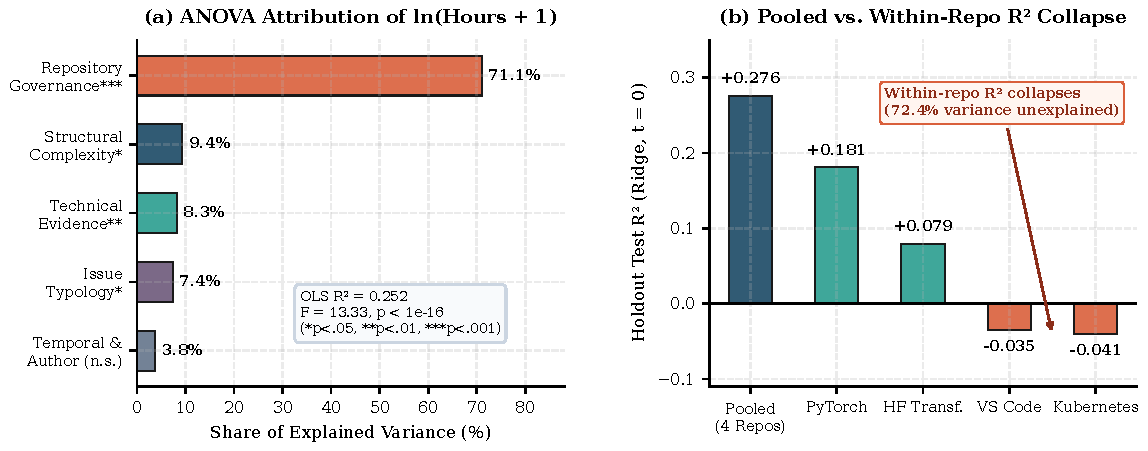
\includegraphics[width=0.92\textwidth]{fig4_resolution_feasibility.pdf}
    \caption{Econometric proof of resolution-time predictability limits ($t=0$ features only). (a) Type-III ANOVA decomposition of OLS on $\ln(\text{hours}+1)$ proves that repository governance drives $71.11\%$ of explainable variance. (b) Consequently, while pooled Ridge regression appears moderately predictive ($R^2=+0.276$), within-repository $R^2$ collapses to $[-0.041, +0.181]$, rendering exact-hour creation-time forecasts scientifically unreliable.}
    \label{fig:resolution}
\end{figure*}

Fitting a multivariate OLS model on $\ln(\text{hours}+1)$ with all $28$ strictly creation-time ($t=0$) predictors yields $R^2 = 0.2523$ (adjusted $R^2 = 0.2334$, $F = 13.33$, $p < 10^{-16}$), with homoskedastic residuals (Breusch--Pagan $p = 0.1274$) and near-normal Omnibus diagnostics ($p = 0.0711$). Crucially, Type-III ANOVA variance decomposition (Fig.~\ref{fig:resolution}(a)) reveals that \textbf{Repository Governance alone accounts for $71.11\%$ of all explainable variance} ($F=45.27$, partial $\eta^2 = 0.1094$), dwarfing Structural Complexity ($9.38\%$, $p=0.037$), Technical Evidence ($8.28\%$, $p=0.008$), Issue Typology ($7.44\%$, $p=0.015$), and Temporal/Author Context ($3.78\%$, non-significant at $p=0.301$).

\begin{table}[t]
\centering
\caption{Creation-Time ($t=0$) Resolution Prediction Benchmarks ($N=227$ Holdout, 28 Leakage-Free Predictors)}
\label{tab:resolution}
\setlength{\tabcolsep}{3.2pt}
\resizebox{\columnwidth}{!}{%
\begin{tabular}{@{}lcccc@{}}
\toprule
\multicolumn{5}{c}{\textbf{Panel A: Continuous $\ln(\text{hours}+1)$ Regression}} \\
\midrule
\textbf{Model} & \textbf{Test $R^2$} & \textbf{MAE (log)} & \textbf{MAE (h)} & \textbf{Spearman $\rho$} \\
\midrule
Dummy Mean & $-0.0001$ & 1.644 & 187.0 & 0.000 \\
Random Forest & 0.2482 & 1.319 & 167.8 & 0.492 \\
Gradient Boosting & 0.2518 & 1.345 & 169.1 & 0.507 \\
\textbf{Ridge (Pooled)} & \textbf{0.2759} & \textbf{1.391} & \textbf{176.6} & \textbf{0.528} \\
\emph{Within-Repo Range} & $[-0.041, 0.181]$ & $1.21$--$1.73$ & --- & $0.123$--$0.424$ \\
\midrule
\multicolumn{5}{c}{\textbf{Panel B: Discrete 4-Tier Velocity Classification}} \\
\midrule
\textbf{Model} & \textbf{Exact Acc.} & \textbf{Bal.\ Acc.} & \textbf{Mac.\ F1} & \textbf{Adj.\ ($\pm 1$) Acc.} \\
\midrule
Dummy Prior & 38.77\% & 25.00\% & 0.1397 & --- \\
Logistic Regression & 43.17\% & 33.20\% & 0.3271 & --- \\
Gradient Boosting & 47.58\% & 38.28\% & 0.3863 & --- \\
\textbf{Random Forest} & \textbf{51.10\%} & \textbf{39.94\%} & \textbf{0.4032} & \textbf{88.11\%} \\
\bottomrule
\end{tabular}%
}
\end{table}

Table~\ref{tab:resolution} and Fig.~\ref{fig:resolution}(b) demonstrate the decisive practical consequence. On the $N=227$ holdout split, pooled Ridge regression achieves $R^2 = 0.2759$ ($\rho = 0.528$, $p = 1.04 \times 10^{-17}$), yet when evaluated \emph{within each repository}, $R^2$ collapses to $+0.1811$ on \texttt{pytorch}, $+0.0794$ on \texttt{transformers}, and turns \emph{negative} on \texttt{vscode} ($-0.0352$) and \texttt{kubernetes} ($-0.0406$). Over \textbf{$72.41\%$} of variance is governed by unobservable post-creation dynamics (maintainer availability, reproduction cycles, release freezes). Consequently, exact-hour forecasting at $t=0$ creates harmful false precision and must be quarantined from SLA promises. By contrast, framing resolution as coarse 4-tier velocity classification (Random Forest) yields $51.10\%$ exact accuracy ($+12.33$ pp above the $38.77\%$ prior) and \textbf{$88.11\%$ adjacent accuracy ($\pm 1$ tier)} with only $0.44\%$ extreme 3-tier errors. For universal cross-repository analytics, however, even discrete tiers require repository baselines; hence OpenSourceLens anchors production resolution intelligence strictly on empirical \textbf{Kaplan--Meier survival curves} and observed quartiles computed directly from each target repository.

\textbf{Finding 4:} \emph{Repository governance explains $71.11\%$ of explainable $t=0$ resolution variance; pooled regression metrics create a statistical mirage that vanishes within individual projects ($R^2 \le 0.181$). Honest OSS analytics must reject exact-hour predictions in favor of right-censored survival estimators.}

\subsection{RQ5: Live Unseen-Repository Case Studies and Honest Telemetry}
\label{sec:results_live}

To test generalization beyond the four benchmark ecosystems, Table~\ref{tab:live} reports verified snapshot-isolated telemetry persisted from live GitHub API ingestion across three structurally diverse unseen repositories: a commercial open-source TypeScript platform (\texttt{RocketChat/Rocket.Chat}), a mature Python CLI library (\texttt{pallets/click}), and the C-language Git version control system (\texttt{git/git}).

\begin{table*}[t]
\centering
\caption{Live Unseen-Repository Telemetry Under Rate-Budgeted Ingestion and Confidence Accounting (\texttt{v2026.2})}
\label{tab:live}
\setlength{\tabcolsep}{4.0pt}
\resizebox{\textwidth}{!}{%
\begin{tabular}{@{}lcccccccccc@{}}
\toprule
\textbf{Unseen Repository} & \textbf{Lang.} & \textbf{Stars} & \textbf{Gini} & \textbf{BF50 /} & \textbf{PRs /} & \textbf{TTFResp} & \textbf{Merge} & \textbf{Issue} & \textbf{SemVer /} & \textbf{Conf.} \\
 & & \textbf{(k)} & & \textbf{BF80} & \textbf{Merge\%} & \textbf{p50 (h)} & \textbf{p50 (h)} & \textbf{p50 (h)} & \textbf{$\text{CV}_{\text{rel}}$} & \textbf{(Band)} \\
\midrule
\texttt{RocketChat/Rocket.Chat} & TS & 46.5 & 0.469 & 3 / 6 & 101 / 58.3\% & 0.00$^\star$ & 990.48 & \texttt{NULL}$^\ddagger$ & 100\% / 1.50 & 0.850 (High) \\
\texttt{pallets/click} & Py & 17.8 & 0.495 & 1 / 2 & 100 / 45.3\% & 11.16 & 17.48 & 4.88 & 90.3\% / 1.45 & 0.814 (High) \\
\texttt{git/git} & C & 64.4 & 0.731 & 1 / 2 & 300 / 1.1\% & 0.55 & \texttt{NULL} & \texttt{NULL} & \texttt{NULL} & 0.736 (Med.) \\
\bottomrule
\multicolumn{11}{@{}l@{}}{\footnotesize $^\star$Near-instant initial conversation response in bounded snapshot; $^\ddagger$Only $5$ pure issues captured in $10$-req snapshot (flagged \texttt{degraded}).}
\end{tabular}%
}
\end{table*}

These three live runs highlight why statistical guardrails are indispensable across the open-source world:
\begin{enumerate}
    \item \textbf{Governance Divergence (\texttt{git/git}):} Despite $64.4\text{k}$ stars, \texttt{git/git} disables GitHub Issues, disables formal GitHub Releases, and integrates patches through the Git mailing list rather than GitHub's merge button. Consequently, our engine observes a \textbf{$98.9\%$ PR abandonment rate} ($1.1\%$ merged via GitHub), high committer concentration (\textbf{$\text{Gini}=0.731$, $\text{BF}_{50}=1$, top-1 share $71.0\%$} driven by maintainer integration commits), and zero pure GitHub issues. Rather than coercing missing metrics to zero or penalizing Git with a misleading ``unhealthy'' composite score, the engine preserves \texttt{NULL} values, surfaces explicit empty-domain penalties (confidence $0.736$, \emph{medium}), and suppresses cross-domain permutation tests where $K < 12$ overlapping months exist.
    \item \textbf{Maintenance Contrasts (\texttt{click} vs.\ \texttt{Rocket.Chat}):} With just $10$ REST requests (\emph{Fast Snapshot}), \texttt{pallets/click} exposes a compact maintainer core ($\text{BF}_{50}=1$, $\text{top-1 share}=53.0\%$) with brisk turnaround (median PR first response $11.16$\,h, merge $17.48$\,h, issue closure $4.88$\,h) alongside a $60.0\%$ stale open backlog and sporadic release cadence ($\text{CV}_{\text{release}}=1.45$, $90.3\%$ SemVer). By contrast, \texttt{RocketChat/Rocket.Chat} exhibits broader contributor distribution ($\text{Gini}=0.469$, $\text{BF}_{50}=3$, $\text{BF}_{80}=6$), strict SemVer adherence ($100\%$), and substantially longer PR merge latency ($p_{50}=990.48$\,h) reflecting enterprise review cycles.
\end{enumerate}

\textbf{Finding 5:} \emph{Applying uniform popularity metrics or unguarded averages across unseen OSS ecosystems systematically misinterprets external-workflow projects such as \texttt{git/git}. Explicit \texttt{NULL} preservation, bounded-sample confidence penalties, and temporal overlap gates enable honest, workflow-aware diagnosis within a $10$--$50$ API request budget.}

% ============================================================================
\section{Threats to Validity and Limitations}
\label{sec:threats}
% ============================================================================

\textbf{Construct Validity.} Canonical label mapping consolidates heterogeneous repository labels into five classes; however, \texttt{other} aggregates diverse maintenance, CI, and meta-tracking tasks, which accounts for $96.84\%$ of DistilBERT's errors and contributes to LORO divergence on Kubernetes. Similarly, our retrieval benchmark ($N=120$) pairs explicit cross-references with textual perturbations; longitudinal human-verified duplicate logs would further strengthen recall validation.

\textbf{Internal Validity.} All resolution predictors were audited to prevent post-creation leakage ($t=0$ only), yet GitHub issue templates sometimes evolve over a repository's history. For live ingestion, \emph{Fast Snapshot} ($10$ requests) and \emph{Standard Diagnostic} ($50$ requests) deliberately bound temporal depth to respect public API quotas; consequently, longitudinal cross-domain permutation pairs ($K \ge 12$ months) and full-history contributor retention cohorts are properly suppressed rather than extrapolated from truncated windows.

\textbf{External Validity.} While our offline benchmark spans four major ecosystems across Go, Python, C++, and TypeScript ($N=2{,}328$), extreme minority sparsity on \texttt{documentation} ($17$) and \texttt{question} ($4$) limits five-class recall on those rare categories. Expanding the labeled LORO corpus across $20+$ mid-sized and domain-diverse repositories remains essential future work. Additionally, live empirical evaluations in this study ran on SQLite in WAL mode; high-concurrency multi-worker throughput on PostgreSQL remains to be stress-tested at production scale.

% ============================================================================
\section{Conclusion and Future Work}
\label{sec:conclusion}
% ============================================================================

This paper empirically examined the foundational reliability limits of automated analytics and machine learning across open-source software ecosystems. Moving beyond surface-level vanity counters requires pairing rate-budgeted telemetry acquisition with strict statistical discipline---snapshot isolation, right-censored survival estimation, non-zero coercion, lag-1 autocorrelation and FDR screening, and explicit confidence penalties.

Our multi-ecosystem experiments establish four actionable principles for empirical software engineering and OSS data science: (1) full-document calibrated lexical models outperform $256$-token transformers on verbose GitHub bug reports while running $42\times$ faster on CPU, because log truncation disproportionately degrades attention windows; (2) strict Leave-One-Repo-Out evaluation is mandatory to expose cross-project taxonomy shift, and calibrated abstention substantially recovers OOD precision; (3) compact $384$-dimensional dense sentence embeddings stored as native relational BLOBs outperform lexical duplicate retrieval with a zero-noise duplicate band at $\cos \ge 0.70$; and (4) because repository governance accounts for $71.11\%$ of explainable $t=0$ resolution-time variance and within-repository regression collapses ($R^2 \le 0.181$), exact-hour SLA prediction should be replaced by empirical Kaplan--Meier survival curves.

Future work will investigate long-context and hierarchical encoders ($>1{,}024$ tokens) to resolve verbose stack-trace truncation, expand multi-ecosystem LORO corpora with balanced minority labels and domain-adaptive calibration for specialized governance dialects such as Kubernetes, and implement incremental full-history synchronization to unlock longitudinal retention cohorts and cross-domain monthly permutation discovery at scale.

\bibliographystyle{IEEEtran}
\bibliography{references}

\end{document}
